\section{Programmeren}

\frame{ \tableofcontents[currentsection] }

\begin{frame}
  \frametitle{CPUs}
  \begin{center}
    \begin{tikzpicture}[cpu/.style={rectangle,thin,fill=gray,opacity=.5,text opacity=1},
                        talk/.style={rectangle,opacity=.75,text opacity=1},
                        franca/.style={shape=ellipse,fill=yellow,opacity=.5,text opacity=1},
                        translate/.style={->,ultra thick,brown}]
      \path[use as bounding box] (-3,-3) rectangle (3, 3);

      \foreach \angle / \file in { 0/intel, 72/arm, 144/ultrasparc, 216/cell, 300/itanium} {
        \node (\file) at (\angle:3) { 
           \pgfimage[width=2cm,interpolate=true]{\file.jpg}
        };
      }

      \only<2->{
        \node[cpu] [below of=intel,yshift=-1mm] { \tiny Desktops/Laptops };
        \node[cpu,yshift=-3mm] [below of=arm] { \tiny Smartphones };
        \node[cpu] [below of=ultrasparc,yshift=-3mm] { \tiny Servers };
        \node[cpu] [below of=cell,yshift=-3mm] { \tiny PlayStation 3 };
        \node[cpu] [below of=itanium] { \tiny Servers };
      }

      \only<3->{
        \node[talk,fill=green] at (0:3) { Hello, there };
        \node[talk,fill=red] at (72:3) { Comment allez-vous? };
        \node[talk,fill=blue] at (144:3) { Vamos a la playa };
        \node[talk,fill=orange] at (216:3) { Jawohl! };
        \node[talk,fill=purple] at (300:3) { Ik begrijp u niet };
      }

      \only<4>{
        \node[franca] (lf) at (0, 0) {Lingua Franca};
        \draw[translate] (lf) to [bend right=30] (intel);
        \draw[translate] (lf) to [bend right=30] (arm);
        \draw[translate] (lf) to [bend right=30] (ultrasparc);
        \draw[translate] (lf) to [bend right=30] (cell);
        \draw[translate] (lf) to [bend right=30] (itanium);
      }
    \end{tikzpicture}
  \end{center}
\end{frame}

\begin{frame}
  \frametitle{Programmeertalen}
  \begin{center}
    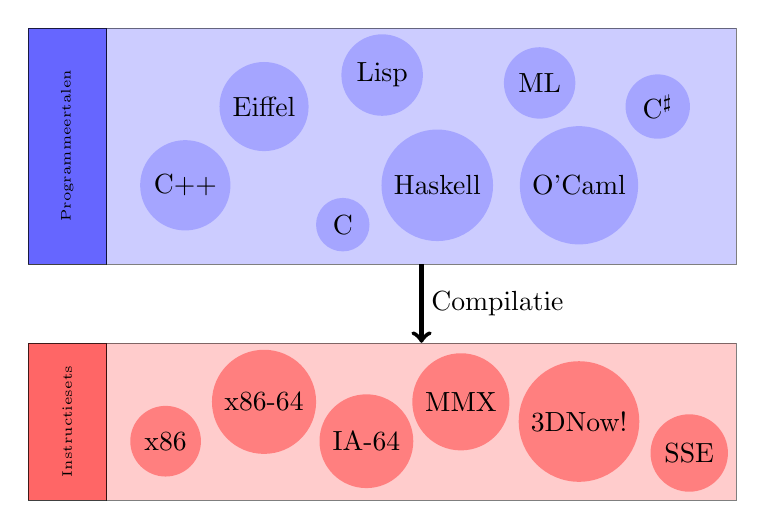
\begin{tikzpicture}[lang/.style={circle,fill=blue!50,opacity=.5,text opacity=1},
                        asm/.style={circle,fill=red!80,opacity=.5,text opacity=1},
                        translate/.style={->,ultra thick,black}]
      \draw[fill=blue!40,opacity=.5,ultra thin] (0, 3) rectangle ++(8, 3);
      \draw[fill=blue!80,opacity=.75,ultra thin] (-1, 3) rectangle ++(1, 3);
      \node[rotate=90] at (-0.5,4.5) { \tiny Programmeertalen };

      \draw[fill=red!40,opacity=.5,ultra thin] (0, 0) rectangle (8, 2);
      \draw[fill=red!80,opacity=.75,ultra thin] (-1, 0) rectangle (0, 2);
      \node[rotate=90] at (-0.5,1) { \tiny Instructiesets };

      \node[lang] at (1,4) {C++};
      \node[lang] at (2,5) {Eiffel};
      \node[lang] at (3,3.5) {C};
      \node[lang] at (4.2,4) {Haskell};
      \node[lang] at (6,4) {O'Caml};
      \node[lang] at (7,5) {C$^\sharp$};
      \node[lang] at (5.5,5.3) {ML};
      \node[lang] at (3.5,5.4) {Lisp};

      \node[asm] at (.75,.75) {x86};
      \node[asm] at (2,1.25) {x86-64};
      \node[asm] at (3.3,.75) {IA-64};
      \node[asm] at (4.5,1.25) {MMX};
      \node[asm] at (7.4,0.6) {SSE};
      \node[asm] at (6,1) {3DNow!};

      \draw[translate] (4,3) -- (4,2);
      \node[anchor=west] at (4, 2.5) { Compilatie };
    \end{tikzpicture}
  \end{center}
\end{frame}


\begin{frame}
  \frametitle{Bijkomend Probleem: Besturingssystemen}
  \structure{Intel}
  \begin{columns}
    \column{.5\textwidth}
    \begin{itemize}
      \item Windows
            \begin{itemize}
              \item Windows 3.1
              \item Windows 95
              \item Windows 98
              \item Windows Me
              \item Windows 2000
              \item Windows XP
              \item Windows Vista
              \item Windows 7
              \item Windows 8
              \item \dots
            \end{itemize}
    \end{itemize}
    \column{.5\textwidth}
    \begin{itemize}
      \item DOS
            \begin{itemize}
              \item MS-DOS 1.0--8.0
              \item IBM PC DOS
              \item Novell Dos
              \item DR DOS
            \end{itemize}
      \item Linux
      \item MacOS
      \item FreeBSD
      \item BeOS
      \item OS/2
  \end{itemize}
  \end{columns}
\end{frame}

\begin{frame}
  \frametitle{Platform}
  \structure{Probleem}
  \begin{itemize}
    \item Platform = CPU + Besturingssysteem
    \item CPUs hebben verschillende instructieset
    \item Besturingssystemen bieden verschillende diensten
    \item Programma's moeten specifiek voor platform gemaakt worden
  \end{itemize}
  \vskip5mm
  \structure{Resultaat}
  \begin{center}
    Meerdere platforms ondersteunen \\ $\Downarrow$ \\ Meermaals zelfde programma herschrijven
  \end{center}
\end{frame}

\begin{frame}
  \frametitle{Emulatoren}
  \structure{Wat is een emulator?}
  \begin{itemize}
    \item Een emulator is software die toelaat om een programma geschreven voor platform X
          te doen draaien op platform Y
  \end{itemize}
  \vskip4mm
  \structure{Voorbeelden}
  \begin{itemize}
    \item ePSXe: PlayStation spellen op Android/Windows/Linux
    \item No\$GBA: GameBoy, GBA, DS spellen op Mac, Linux, PC, Wii
    \item DOSBOX: DOS programma's op Windows, BeOS, Linux, MacOS, OS/2
  \end{itemize}
\end{frame}

\begin{frame}
  \frametitle{Java}
  \begin{itemize}
    \item Java definieert een nieuw \emph{platform}
          \begin{itemize}
            \item Eigen instructieset (Java Bytecode)
            \item Eigen ``diensten'' (Java API)
          \end{itemize}
    \item Java is een \emph{virtueel} platform
          \begin{itemize}
            \item Er is geen Java CPU
            \item Er is geen Java OS
          \end{itemize}
    \item Java wordt ge\"implementeerd \emph{bovenop andere platforms}
          \begin{itemize}
            \item Java Virtual Machine is de emulator
            \item JVM vertaalt Java Bytecode naar juiste instructieset
            \item Doet beroep op onderliggend OS
          \end{itemize}
    \item $\Rightarrow$ Een Java programma is \emph{platformonafhankelijk}
          \begin{itemize}
            \item Java programma's werken voor ieder platform waarvoor een JVM bestaat
          \end{itemize}
  \end{itemize}
\end{frame}

\begin{frame}
  \frametitle{Java}
  \begin{center}
    \begin{tikzpicture}[java/.style={rectangle,fill=blue!50,minimum width=100mm,minimum height=8mm,drop shadow},
                        bytecode/.style={rectangle,fill=blue!50,minimum width=100mm,minimum height=8mm,drop shadow},
                        jvm/.style={rectangle,fill=blue!50,minimum width=100mm,minimum height=8mm,drop shadow},
                        jvmi/.style={rectangle,fill=blue!50,minimum width=15mm,minimum height=15mm,drop shadow},
                        arr/.style={->,ultra thick}]
      \node[java] (java program) at (0,5) {Java Programma (.java)};
      \node[bytecode] (java bytecode) at (0,3.5) {Java Bytecode (.class)};
      \node[jvm] (jvm) at (0,2) {Java Virtual Machine};

      \foreach \file / \pos in {windows/0,linux/2,macos/-2,freebsd/4,beos/-4} {
        \node[jvmi] (\file) at (\pos,0) {\pgfimage[height=1cm,interpolate=true]{\file}};        
        \draw[arr] (\file.north |- jvm.south) -- (\file.north);
      }

      \draw[arr] (java program) to node [auto] {{\tt javac}} (java bytecode);
      \draw[arr] (java bytecode) to node [auto] {{\tt java}} (jvm);
    \end{tikzpicture}
  \end{center}
\end{frame}

\begin{frame}
  \frametitle{Demo}
  \codeblock{helloworld.java}{Hello World}
  \begin{itemize}
    \item Open notepad en typ bovenstaande code over
    \item Bewaar in \X{\tt MyApp.java}{filename}
    \item Open console ({\tt cmd.exe})
    \item \X{\tt javac MyApp.java}{javac}
    \item \X{\tt java MyApp}{java}
  \end{itemize}
  
  \begin{tikzpicture}[overlay,
                      remember picture,
                      msg/.style={rectangle,fill=blue!50,opacity=.75,text opacity=1,drop shadow},
                      arr/.style={->,thick}]
    \only<2>{
      \node[msg] (msg filename) at (8, 1) {\parbox{5cm}{\raggedright Bestandsnaam moet zelfde naam hebben als klasse}};
      \draw[arr] (msg filename.north) to [bend right=30] (MyApp);
      \draw[arr] (msg filename.west) to [bend left=30] (filename.south);
    }
    \only<3>{
      \node[msg] (msg javac) at (8, 1) {\parbox{5cm}{\raggedright Vertaalt code naar bytecode en bewaart het in {\tt MyApp.class}}};
      \draw[arr] (msg javac.west) to [bend left=30] (javac.south east);
    }
    \only<4>{
      \node[msg] (msg java) at (8, 1) {\parbox{5cm}{\raggedright Start de JVM op en voert je programma uit}};
      \draw[arr] (msg java.west) to [bend left=30] (java.south east);
    }
  \end{tikzpicture}
\end{frame}

\begin{frame}
  \frametitle{Java Installeren}
  \structure{JRE}
  \begin{itemize}
    \item Java Runtime Environment
    \item Bevat Java Virtual Machine
    \item Geen compiler
    \item Bestemd voor \emph{gebruikers} van Java programma's
  \end{itemize}
  \vskip4mm
  \structure{JDK}
  \begin{itemize}
    \item Java Development Kit
    \item Bevat Java Virtual Machine
    \item Bevat compiler (en vele andere tools)
    \item Bestemd voor \emph{programmeurs}
    \item \url{http://www.oracle.com/technetwork/java/javase/downloads/index.html}
  \end{itemize}
\end{frame}

\begin{frame}
  \frametitle{Integrated Development Environment (IDE)}
  \begin{itemize}
    \item Notepad + {\tt javac} niet erg praktisch
    \item IDE: ontwikkelomgeving
    \item Biedt veel extra ondersteuning
          \begin{itemize}
            \item Automatische compilatie
            \item Syntax highlighting
            \item On the fly errors
            \item AutoComplete
            \item Debugging
            \item \dots
          \end{itemize}
    \item Meerdere beschikbaar
          \begin{itemize}
            \item \href{http://www.eclipse.org}{\beamergotobutton{Eclipse}}
            \item \href{https://netbeans.org/}{\beamergotobutton{NetBeans}}
            \item \href{http://www.jetbrains.com/idea/}{\beamergotobutton{IntelliJ}}
            \item \dots
          \end{itemize}
  \end{itemize}
\end{frame}



%%% Local Variables: 
%%% mode: latex
%%% TeX-master: "intro"
%%% End: 
